\chapter{BACKGROUND AND RELATED WORK}

In this chapter, we review some of the
associated topics which are pertinent to the
research performed in this dissertation.
Accordingly, we present background and related
work in the areas of wireless sensor networks
(WSN) middleware, resource management in WSN and
sparse WSN. We also provide a brief introduction
to reinforcement learning (RL), multi-agent
systems and collective intelligence (COIN)
theory which plays significant role in our work. 

\section{Wireless Sensor Networks Middleware}

Complexity of sensor network applications is
continuously increasing with the proliferation of
distributed computing and wireless connectivity
in sensor networks. Heterogeneity of sensor
networks in terms of hardware characteristics as
well as application requirements further adds on
application complexity. As a result, developing
sensor network applications has become very
difficult. A middleware infrastructure is
required which can ease up scuh application
development. Challenges faced by WSN applications
and requirement and design principles of a
middleware emerging out of those challenges are
discussed next.

\subsection{WSN Middleware Challenges}
Development and implementation of a sensor
network middleware is not a trivial
task and the main reason for this is some inherent
characteristics of wireless sensor networks. We
have tried to capture some of these
characteristics here.
\begin{itemize}
	\item Sensor nodes are limited in amount of
	energy they can store or achieve from the
	environment. This size and energy limit implies
	extremely resource constrained devices in terms
	of CPU power, memory and wireless bandwidth and
	range which in turn limits processing and
	interactions normally required by distributed
	systems.
	\item Sensor nodes are subject to failures more
	regularly either due to depletion of battery or
	environmental influences. Also nodes can be
	highly mobile. this brigns in high degree of
	dynamics and uncertainty in WSN and can result
	in frequent topology changes and network
	partitions.
	\item Wireless link used by low power sensor
	nodes is also normally error prone. Hence
	communication failure is also a problem to be
	addressed. 
	\item WSN is often heterogeneous, e.g. a network
	often consists of nodes/devices with various
	capabilities in terms of sensors, computing
	power and memory. This further complicates
	WSN management.
	\item A WSN application consisting of hundreds
	or even thousands of sensor nodes is normal and
	hence scalability is a major issue here.
	\item Large number of sensor nodes and
	possibility of their deployment in hostile or
	in-accessible area mandates that such a system
	provides \quote{exception-free unattended
	operation} \cite{Estrin99}. This suggests the
	necessity of autonomous adaptation in terms of re-programmability and task dynamics.
	\item Concern for security and privacy is more
	aggravated for WSN applications because of
	sensitiveness of data collected and lack of
	resources. 
	\item With the pervasiveness of sensor network
	applications, it will become necessary to
	support multiple heterogeneous applications with
	different requirements on top of single network.
\end{itemize}

\subsection{WSN Middleware Requirements}
Above challenges can be interpreted to frame a
list of requirements for WSN middleware. This
list is as follows:
\begin{itemize}
  \item Middleware system should support
  high level abstraction hiding complexity of 
 dealing with individual node and provide a
 holistic view of the network. Middleware should
 multiple programming paradigms like
 publish-subscribe, pull-push models, event based
 etc.
 \item It is necessary for WSN middleware to be
 very efficient in terms of energy, bandwidth and
 computational resources consumption. 
 \item Middleware should be proactive and support
 adaptive fidelity algorithms to improve
 performance.
 \item Middleware should be able to provide
 support for programmability i.e. deployment,
 configuration and reconfiguration. It should
 also provide mechanisms for application policy
 creation and distribution.
 \item WSN middleware needs to provide
 scalability in terms of number of sensor nodes,
 applications running on top of it and associated
 users.
 \item Middleware needs to support execution of
 multiple applications simultaneously on a single
 sensor network. It should be able to support QoS
 requirements of individual application in terms
 of availability, timeliness, fault-tolerance etc.
 \item WSN middleware should be able to provide
 optimal network configurations in order to
 support high degree of dynamics of WSN. 
 \item It should provide security in context of
 data processing, data communications, device
 tampering etc.
 \item Finally, middleware itself should be
 lightweight in terms of computation and
 communciation requirements in order to be
 successful in resource constraint wireless
 sensor networks.
\end{itemize}

\subsection{WSN Middleware Design Principles}
Based on some previous work \cite{Estrin99,Yu04},
we have hereby listed some design principles to
aid in design of middleware fulfilling above
requirements.
\begin{itemize}
  \item A WSN middleware framework should support
  the data-centric or data-driven model for data
  processing and querying.
  \item A WSN middleware should allow
  incorporation of application knowledge and
  hence allow overall software to be tailored to
  the executing application. This conflicts with
  desire to support and optimize for a wide class
  of applications. Hence a trade-off is required
  between application specification and
  generality of the middleware. This is most of
  the time resolved by allowing application to
  put its unique features as code or
  specification which can be interpreted by
  middleware.
  \item Cluster-based localized algorithms should
  be used for efficiently coordinating local
  interactions between sensor nodes in order to
  achieve global goals. This can help in creating
  more scalable applications and can improve
  robustness and efficiency in resource
  utilization.
  \item Middleware should should support various
  \emph{data reduction techniques} required for
  colection and processing of sensory data.
  Complex sensing tasks often require that data
  collected at many nodes be fused to obtain a
  high-level sensing result. For reducing
  communication and energy overhead, it is
  necessary to process sensory data at source to
  extract relevant features. Middleware will
  require means to specify application knowledge
  and ways to inject this knowledge into the
  nodes of the network.
  \item Sensor networks are mostly connected to
  external background infrastructures mainly for
  tasking the sensor network, as well as for
  evaluation and storage of sensing results and
  also may provide computing and storage
  resources not available to sensor networks.
  Hence, middleware should allow the integration
  with such background infrastructures, providing
  a homogeneous view of the entire system.
\end{itemize}

\subsection{WSN Middleware Classification}
\begin{figure}[tbp]
\centerline{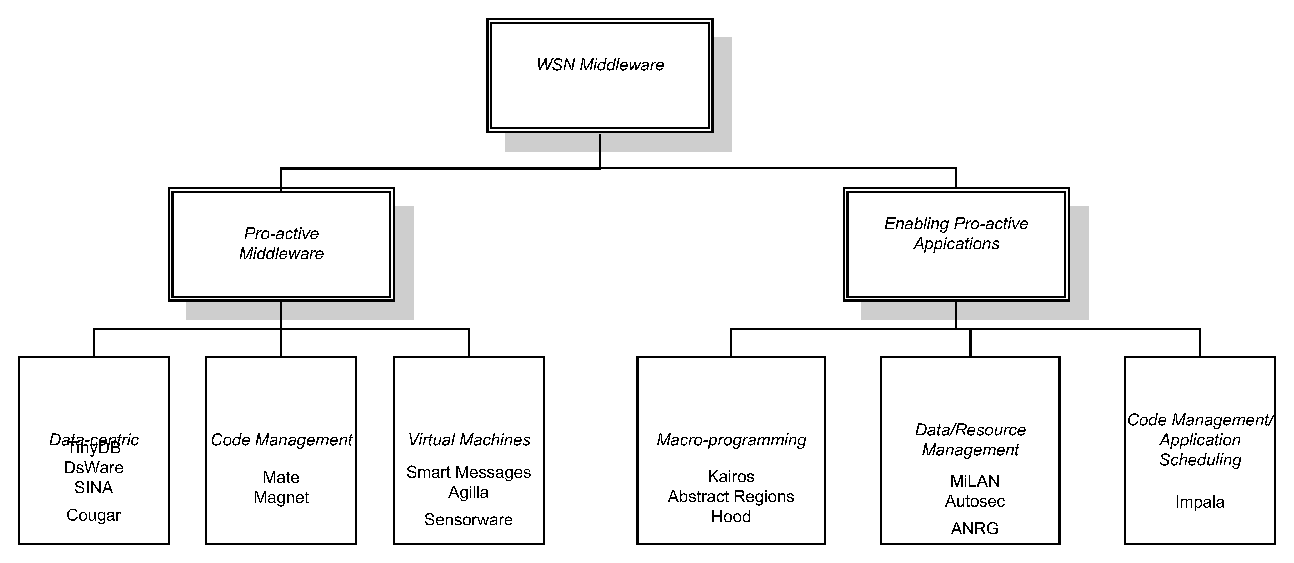
\includegraphics[width=4in]{figures/middleware-classification.eps}}
\caption{WSN Middleware Classification}
\label{fig:middleware-classification}
\end{figure}
A high level classification of the WSN 
middleware frameworks is given in Figure
\ref{fig:middleware-classification}. As
shown in the figure, WSN middleware can be
broadly classified into pro-active middleware
and middleware enabling pro-active applications
\cite{Heinzelman04}. Pro-active middleware refers
to middleware that pro-actively changes WSN
functionality based on current environment and
state of the system. On the other side,
middleware enabling pro-active applications
allows application to guide system on how to
adapt to changes in the environment and state of
the system. 
Pro-active middleware can be further classified
into the following:
\begin{itemize}
  \item \emph{Data-centric}: Middleware in this
  category provides the abstraction of the   whole
  sensor network as a virtual   distributed
  database. Idea is to enable   utilization of
  higher level declarative   programming
  language/interface upon the   distributed nodes
  without having to deal with the network issues.
  User dispatches queries using some easy-to-use
  interface to extract data of interest. The main
  focus of this type of middleware is on efficient
  evaluation of query plans using in-network query
  processing. Such middleware normally only uses
  predefined static task schedules and normally
  doesn't handle adaptive task/resource management.
  Also the approach provides only approximate
  values and lacks support for real-time
  applications that need spatio-temporal
  relationships between events\cite{Hadem06}.This
  type of middleware are not expressive enough
  to implement arbitrary distributed algorithms.
  Cougar \cite{Yao02} is the first work considering WSN as a database. TinyDB \cite{Madden02} hides the complexity of TinyOS by building
  query-processing system on top of it. TinyDB
  allows users to extract data of interest of the
  sensor nodes using a SQL-like interface.
  SINA\cite{Srisathapornphat01} and
  DsWare\cite{Son03} are other two approaches
  falling into this category of middleware using
  database abstraction.
  \item  \emph{Code Management}:
\end{itemize}
\subsection{}
There are many proposed middleware solutions for WSNs that have ad-
vocated strong need for proactive adaptation of resources [3, 4, 5]. MiLAN
[3] gets QoS requirements and sensor
confgurations from the application and adapts the network conguration and other sensor resources e.g. which sensor
should send data and which should act as a router etc. A cluster-based archi-
tecture is described in [4] using virtual-machine abstraction where each cluster
consists of a set of spatially adjacent sensor nodes that cooperate together to
create an adaptive resource management layer. TinyCubus [5] consists of a
data management framework that aims at providing adaptation of system and
data management components at runtime based on application requirements
3
and system parameters. Even though the issue of enabling adaptive resource
management for WSN applications is addressed, the above-mentioned solutions
require complete knowledge of the system as well as some kind of cooperation
among sensor nodes. Hence they may not be directly relevant to data-collection
application in sparse network with mobile elements.
To the best of our knowledge, there are only a few middleware solutions
explicitly targeted to wireless sensor networks with mobile elements. Among
them, the Impala [6] middleware architecture has been proposed for application
adaptation and update. Impala is built on top of an event-based programming
model. As for adaptation, it provides a mechanism for dynamically querying
operating parameters and checking them against a set of rules to determine
if an application switch is required. Application
switching is based on a finite state machine
model, where transitions are defined in the form
of heuristics, and can cope with device failures.
However, Impala has been specifically targeted to scenarios where all nodes are mobile and act as peers. In addition, the focus is more on application adaptation and update, rather than on resource
allocation. More recently, the TinyLime [7] middleware has been proposed for
the specific scenario of sparse WSNs. TinyLime
is based on a tuple space model, an implementation of the distributed shared memory paradigm for distributed
computing. The original tuple space model is extended to the scenario where
multiple MDCs collect data from sensor nodes which are not densely deployed in
the network. To this end, no assumption is made on network connectivity, since
nodes can even be isolated from each other. TinyLime provides mechanisms to
perform data aggregation and tune the activity of nodes in order to save energy.
However, the focus of TinyLime is on their proposed programming abstraction
rather than on adaptation and resource management. On the contrary, in this
paper we propose and adaptive middleware approach to resource allocation for
energy-efficient and reliable data collection in
sparse WSNs. \section{Resource Management in Wireless Sensor
Networks}

%Market/economics based, AI based,
% centralized/distributed,
% coin

\section{Reinforcement Learning}
%Q-learning, MAS, RL based MAS, COIN

\section{Sparse WSN}
